\documentclass[conference]{IEEEtran}
\IEEEoverridecommandlockouts
% The preceding line is only needed to identify funding in the first footnote. If that is unneeded, please comment it out.
\usepackage{cite}
\usepackage{amsmath,amssymb,amsfonts}
\usepackage{algorithmic}
\usepackage{graphicx}
\usepackage{hyperref}
\usepackage{textcomp}
\usepackage{xcolor}
\usepackage{listings}
\usepackage{lipsum}
\usepackage{eurosym}
\usepackage{soul}
\usepackage{color}

\DeclareRobustCommand{\hlcyan}[1]{{\sethlcolor{cyan}\hl{#1}}}

\colorlet{punct}{red!60!black}
\definecolor{background}{HTML}{EEEEEE}
\definecolor{delim}{RGB}{20,105,176}
\colorlet{numb}{blue!60!black}

\lstdefinelanguage{json}{
	basicstyle=\normalfont\ttfamily,
%	numbers=left,
%	numberstyle=\scriptsize,
%	stepnumber=1,
%	numbersep=8pt,
%	showstringspaces=false,
%	breaklines=true,
%	frame=lines,
%	backgroundcolor=\color{background},
	literate=
	*{0}{{{\color{numb}0}}}{1}
	{1}{{{\color{numb}1}}}{1}
	{2}{{{\color{numb}2}}}{1}
	{3}{{{\color{numb}3}}}{1}
	{4}{{{\color{numb}4}}}{1}
	{5}{{{\color{numb}5}}}{1}
	{6}{{{\color{numb}6}}}{1}
	{7}{{{\color{numb}7}}}{1}
	{8}{{{\color{numb}8}}}{1}
	{9}{{{\color{numb}9}}}{1}
	{:}{{{\color{punct}{:}}}}{1}
	{,}{{{\color{punct}{,}}}}{1}
	{\{}{{{\color{delim}{\{}}}}{1}
	{\}}{{{\color{delim}{\}}}}}{1}
	{[}{{{\color{delim}{[}}}}{1}
	{]}{{{\color{delim}{]}}}}{1},
}


\def\BibTeX{{\rm B\kern-.05em{\sc i\kern-.025em b}\kern-.08em
    T\kern-.1667em\lower.7ex\hbox{E}\kern-.125emX}}
\begin{document}

\title{ArduECO: cheap air quality control for cities}

\author{\IEEEauthorblockN{Voinea Stefan Ciprian}
\IEEEauthorblockA{\textit{University of Padova, Italy} \\
\textit{Department of Pure and Applied Mathematics}\\
	%Padova, Italy \\
	stefanciprian.voinea@studenti.unipd.it}
	%\and
	%\IEEEauthorblockN{2\textsuperscript{nd} Given Name Surname}
	%\IEEEauthorblockA{\textit{dept. name of organization (of Aff.)} \\
	%\textit{name of organization (of Aff.)}\\
	%City, Country \\
	%email address or ORCID}
}

\maketitle

\begin{abstract}
	\lipsum[1]
\end{abstract}

\vspace{.2cm}

\begin{IEEEkeywords}
Arduino, embedded, air-quality
\end{IEEEkeywords}

\section{Introduction}\label{intro}
	More and more people around the world have started to understand the importance of air quality and how much having clean and pollution-free air can influence our lives, both on the small and large scale. 
	To have clean air, all of us have to do something to avoid polluting it. \\
	The Government of Luxembourg has set a good example becoming the first country to offer nationwide free public transport to the citizens\cite{luxemburg}.\\
	For short commutes, vehicles like the classic bike\cite{bike}, the infamous skateboard and the scooter have started to arise and conquer cities, either in their battery-powered or old-school human-powered.\\
	Since not everyone necessarily owns one of these green methods of transportation, companies like \textit{Mobike}\cite{mobike} and \textit{MiMoto}\cite{mimoto} have seen the opportunity to enter the market of shared transportation, proposing a \textit{pay-per-use} solution for bikes, electric scooters and other similar vehicles.	
	Each company has its own application, network infrastructure and smart devices aboard their vehicles, gathering data like GPS (Global Positioning System) position, time spent by the user, parking spot, etc. to send it in the cloud and compute information like cost of the ride and charging it to the user.\\
	All this falls under the \textit{IoT} (Internet of Things) paradigm, which has become a well-described market with new ideas and business opportunities being presented every day.\\
	Among the data collected by these companies, none is about air pollution.\\
	In this article, I describe \textit{ArduECO}, a wireless device based on an Arduino-like board capable of gathering data from previously named vehicles and sending it to the cloud, to be processed and displayed.\\
	%TODO completare
	This paper is organized as follows:
	\begin{itemize}
		\item Section 2: Background and description of the problem
		\item Section 3: State of the art on smart devices that allow tracking pollution
		\item Section 4: implementation of the proposed solution
		\item Section 5: Conclusions
	\end{itemize}

\section{Background problem}
% \subsection{Maintaining the Integrity of the Specifications}
Background

spiegare quali sono le particelle di inquinamento nell'aria

spiegare quali sono i sensori presenti sul mercato che possono rilevarle

tabella con sensori mq e differenze

come mai la scelta di implementarlo in quel modo

\section{State of the art}
	% \subsection{Abbreviations and Acronyms}\label{AA}
	State of the art non solamente della letteratura ma anche di quello che viene offerto sul mercato
	
	\begin{figure}[htbp]
		\centerline{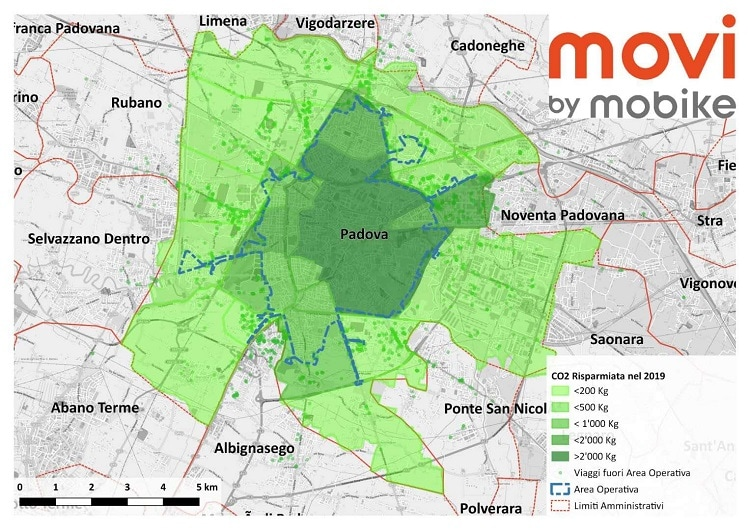
\includegraphics[width=8cm]{fig3.jpg}}
		\caption{Example of a figure caption.\cite{bibid}}
		\label{fig}
	\end{figure}


% DARE DEFINIZIONE DI OPEN SOURCE DA QUALCHE PARTE?
\section{Proposed solution}\label{solution}
	
	ArduECO is a wireless IoT device that represents one of the possible combinations of open source hardware and software.
	% DIRE COSA EFFETTIVAMENTE VIENE CATTURATO, COSA CHE DEVE ESSERE DISCUSSA NEL PARAGRAFO PRECEDENTE
	\hlcyan{This wireless device is able to detect substances in the air and send the data in the cloud over Wi-Fi, and combined with data from other similar devices detect the level of pollution in the air.}\\
	The schematics for this project have been designed using Fritzing, a CAD (Computer-Aided Design) software for the design of electronics hardware\cite{fritzing} and can be seen in Fig.~\ref{schematics}.
	Both code and schematics for this device are available on the GitHub repository ``ArduECO''\cite{ardueco_git}.\\
	Schematics for other components can be easily found online from various sources and vendors: here, for example are the schematics for the MQ7 sensor from SparkFun\cite{spark_mq} and the NodeMCU\cite{node_scheme}.
	
	\subsection{The circuit}\label{circuit}
	
		ArduECO is composed by four main components:
		\begin{itemize}
			\item \textit{NodeMCU}: it's the hearts and brains of the device, this board is an open-source development kit based on the ESP8266 chip that allows for prototyping of IoT devices;
			\item \textit{MicroSD card reader}: this allow for collecting and keeping data cached for the current ride and permanently on a removable memory card;
			\item \textit{GPS sensor}: this allows for localizing the device, it has an onboard LED that blinks when it has established communication with the satellites;
			% AGGIUNGERE COSA RACCOGLIE ESATTAMENTE QUESTO SENSORE
			\item \hlcyan{\textit{MQ sensor}: the MQ sensor used in this project is MQ7 but it can easily be exchanged with other sensors that use the same board and connectors.}
		\end{itemize}
		The other components, LEDs and button, are used as I/O for interacting with the user.\\
		In Section \ref{improvements} I explain how the project can be improved both in hardware and software.
		\begin{figure}[htbp]
			\centerline{
\includegraphics[width=8cm]{fig1.png}}
			\caption{ArduECO schematics}
			\label{schematics}
		\end{figure}
		In Fig.~\ref{schematics} there is no indication of a power supply since for this prototype version it has been powered using an external battery with a standard output of 5V and 1A.
	
	\subsection{The Arduino software}
	
		% Trasformare in forma passiva
		\hlcyan{For ArduECO I chose to use Arduino's programming language instead of MicroPython}\cite{micropyhton} because of the large community supporting it and the vast interoperability with other boards.\\
		The main functions in the Arduino programming language are ``\textit{void setup()[]}'' and ``\textit{void loop()[]}'': the first one runs a single time when the device boots initializing and setting the initial values while the second one loops consecutively, allowing the program to change and respond.
		ArduECO.ino is the main file executed by the NodeMCU and contains the previously described functions.\\
		In ArduECO's software, the setup function contains the instructions to correctly initialize serial communication with the GPS module, create the files in the SD card, initialize the pin-outs, gather the certificates for communicating with the cloud and create a random id for identifying the ride, since each time the device boots is considered as a single ride.\\
		An important part of the configuration of ArduECO is the file \textit{params.json}:
		\begin{lstlisting}[language=json,firstnumber=1]
    {
	  "ssid" : "",
	  "password" : "",
	  "in_topic" : "",
	  "out_topic" : "",
	  "endpoint" : ""
    }
		\end{lstlisting}
		If this file is not present in the SD card at boot-time and correctly formatted, ArduECO will not end the boot sequence, returning an error and rebooting after 10 seconds.\\
		This file contains configurations such network SSID and password, topics for communicating with the MQTT server and its endpoint (network address).\\
		The loop function contains the instructions that tell the board to acquires a reading of its surroundings every 5 seconds by first detecting if a GPS fix os present and by reading the value from the analog pin connected to the MQ sensor.
		Each read is then appended on two separate text files (\textit{cache\_log.txt} and \textit{perm\_log.txt}) in JSON format. 
		\textit{cache\_log.txt} is created each time ArduECO boots is related to a single session while \textit{perm\_log.txt} contains reads about each ride taken.\\
		Here is an example of a logged loop cycle read:
		\begin{lstlisting}[language=json,firstnumber=1]		
    {
	  "id":"127",
	  "air":"18.22",
	  "lt":"45.39641",
	  "lg":"11.88527",
	  "dt":"50320.12173900",
	  "tpc":"ardueco_proto_01_OUT"
    }
		\end{lstlisting}	
		The external LEDs are used to communicate when the setup sequence has finished correctly with errors as well as for indicating whether the SSID specified in the \textit{params.json} file is in range and if ArduECO is transmitting data.\\
		When the button is pressed, ArduECO searches the list of networks in range for the specified one and, if present, connects to it.
		Afterwards it establishes communication with the MQTT server specified by the endpoint, and sending it a message with the number of messages that will be sent.\\
		Each row of the cache file is then transmitted to the server.\\
		At the end of this sequence the cache file is deleted and created again awaiting new reads.\\
		The other files that implement this project contain specific functions for either setting up the device or connecting the the server.
		
	\subsection{The cloud}
	
		When the button is pressed, ArduECO connects to the access point with the SSID specified in the \textit{params.json} file and sends the contents of \textit{cache\_log.txt} to the cloud, specifically to AWS (Amazon Web Services).
		\textit{IoT core} and \textit{Lambda} are the services that are used for this project.\\
		ArduECO sends data to the MQTT server in IoT core specified as \textit{endpoint} in \textit{params.js}.
		It connects to this server using certificates created in the IoT core console and that are loaded in ArduECO's memory, this means that they are uploaded via the Arduino IDE.\\
		The MQTT (Message Queuing Telemetry Transport) server is designed as a lightweight messaging protocol that uses publish/subscribe operations to exchange data between clients and server, fast in data transmission\cite{mqtt}.\\
		This service in IoT core is connected to a serveress Lambda function written in Python, triggered each time a new messages arrives from ArduECO, which receives the JSON message as a parameter and calls a PHP page on \href{ardueco.altervista.org}{ardueco.altervista.org}, where the front end of the service is hosted.
		Altervista is a free website hosting platform with PHP and MySQL database.
		After being saved in the MySQL database in Altervista is then displayed on the homepage using Google Maps' APIs.
		\begin{figure}[htbp] %TODO cambiare immagine, aggiungere marker in DB
			\centerline{\includegraphics[width=8cm]{fig2.png}}
			\caption{Map with markers and reads from \href{ardueco.altervista.org}{ArduECO}.}
			\label{altervista}
		\end{figure}
	
		Each marker on the map represents a reading and, if clicked on, shows the value read by ArduECO's sensor.\\
		Markers are connected with different colors indicating the ride they belong to.
		
	\subsection{Hardware cost}
	
		Because the components used for this project are open-source, they can be found sold on various websites from many vendors.
		Here are some examples of prices taken from the Chinese e-commerce AliExpress\cite{aliexpress} at the time of writing.
		\begin{itemize}
			\item NodeMCU \footnote{\url{https://it.aliexpress.com/item/32879925927.html}}: $ \sim $ 2\euro
			\item MicroSD car reader \footnote{\url{https://it.aliexpress.com/item/32572793362.html}}: $ \sim $ 0.50\euro
			\item GPS sensor \footnote{\url{https://it.aliexpress.com/item/32836015224.html}}: $ \sim $ 3.5\euro
			\item MQ gas sensor \footnote{\url{https://it.aliexpress.com/item/4000575957425.html}}: $ \sim $ 1\euro
		\end{itemize}
		The total cost of these items amounts to $\sim$ 7\euro, considering shipping and costs of remaining components (cables, LEDs, button, SD card), it can arrive to less than 15\euro.\\
		Note that the indicated prices refer to single pieces and in case of bulk purchases (at least 5 or 10 of each piece) the total cost would be much lower.
	
\section{Results and data analysis}\label{AA}
	\subsection{Test scenarios}

		\subsubsection{Prototype test}

		\subsubsection{Real life implementation}
			% \subsection{Abbreviations and Acronyms}\label{AA}
			State of the art
	
	It make detection by method of cycle high and low temperature, and detect CO when low temperature \cite{mq7}


\section{Future improvements}\label{improvements}
	Since ArduECO is one of many possible implementations that this hardware and software can create, there are various improvements which could bring to a better and more stable device.
	
	\subsection{Hardware improvements}
		Many improvements can be made on the hardware: for example, the circuit described in Section \ref{circuit} has a single air sensor due to the limitation of the NodeMCU and ESP8266 chip that have only one analog input pin.\\
		By connecting the board to an \textit{ADC} (Analog to Digital Converter) it becomes possible to add multiple sensors expanding the analog inputs.
		ADCs convert an analog voltage on a pin to a digital number\cite{adc}.\\
		In order to upgrade the transmission method and use mobile data instead of WiFi (which is limited to 2.4GHz on the NodeMCU) it's possible to switch the board to an Arduino Leonardo or an Arduino Uno.\\
		Modules capable to add mobile connectivity can be found on sites like AliExpress\footnote{\href{https://it.aliexpress.com/item/32963853961.html}{https://it.aliexpress.com/item/32963853961.html}} and does not brig much additional overall cost (in this case $ \sim $ 2\euro).\\
		Given the small dimensions of the components, this project could be easily fitted inside of a custom made box.
		A solution could be to design and 3D print a custom plastic case in which fit the whole device, considering that the air sensor should remain outside of the case and the whole project could be exposed to high levels of humidity (for example in the winter season).\\
		Power is one important issue for IoT devices.
		The prototype described in this essay has been powered using an external battery, but it can be coupled with other energy sources like a dynamo, so that it can be powered by movement of the wheel (in case it's installed on a bike).
	
	\subsection{Software improvements}
		The software can be improved in many ways as well.
		For example a control could be added to check if every message has correctly arrived at the IoT server and, in case of a timeout or an eventual error, the message could be sent again.
		
	\subsection{Cloud services improvements}
		The cloud technologies can be improved too.
		AWS' IoT core could be configured in order to have more MQTT servers based on the devices divided by each city or zone in which the ArduECOs are used.\\
		Another important change would be using an AWS EC2 instance to host the website instead of Altervista.
		This introduces of the instance and 
		
		In the development of this project I was forced by the we server host altervista.org to connect to the database only from within
		
		connections within its domain
		
		i was not able to allow the lambda to insert the data directly in the database, so I was forced to create an intermediate webpage to insert that data
		
		for this reason a possible improvement could be 

\section{Conclusions and future work}
This paper describes the implementation of a wireless IoT system capable to gather data from air and send it to the cloud in order to be analyzed and displayed.

%\subsection{Units}
%\begin{itemize}
%\item Use either SI (MKS) or CGS as primary units. (SI units are encouraged.) English units may be used as secondary units (in parentheses). An exception would be the use of English units as identifiers in trade, such as ``3.5-inch disk drive''.
%\item Avoid combining SI and CGS units, such as current in amperes and magnetic field in oersteds. This often leads to confusion because equations do not balance dimensionally. If you must use mixed units, clearly state the units for each quantity that you use in an equation.
%\item Do not mix complete spellings and abbreviations of units: ``Wb/m\textsuperscript{2}'' or ``webers per square meter'', not ``webers/m\textsuperscript{2}''. Spell out units when they appear in text: ``. . . a few henries'', not ``. . . a few H''.
%\item Use a zero before decimal points: ``0.25'', not ``.25''. Use ``cm\textsuperscript{3}'', not ``cc''.)
%\end{itemize}
%
%\subsection{Equations}
%Number equations consecutively. To make your 
%equations more compact, you may use the solidus (~/~), the exp function, or 
%appropriate exponents. Italicize Roman symbols for quantities and variables, 
%but not Greek symbols. Use a long dash rather than a hyphen for a minus 
%sign. Punctuate equations with commas or periods when they are part of a 
%sentence, as in:
%\begin{equation}
%a+b=\gamma\label{eq}
%\end{equation}
%
%Be sure that the 
%symbols in your equation have been defined before or immediately following 
%the equation. Use ``\eqref{eq}'', not ``Eq.~\eqref{eq}'' or ``equation \eqref{eq}'', except at 
%the beginning of a sentence: ``Equation \eqref{eq} is . . .''
%
%\subsection{\LaTeX-Specific Advice}
%
%Please use ``soft'' (e.g., \verb|\eqref{Eq}|) cross references instead
%of ``hard'' references (e.g., \verb|(1)|). That will make it possible
%to combine sections, add equations, or change the order of ures or
%citations without having to go through the file line by line.
%
%Please don't use the \verb|{eqnarray}| equation environment. Use
%\verb|{align}| or \verb|{IEEEeqnarray}| instead. The \verb|{eqnarray}|
%environment leaves unsightly spaces around relation symbols.
%
%Please note that the \verb|{subequations}| environment in {\LaTeX}
%will increment the main equation counter even when there are no
%equation numbers displayed. If you forget that, you might write an
%article in which the equation numbers skip from (17) to (20), causing
%the copy editors to wonder if you've discovered a new method of
%counting.
%
%{\BibTeX} does not work by magic. It doesn't get the bibliographic
%data from thin air but from .bib files. If you use {\BibTeX} to produce a
%bibliography you must send the .bib files. 
%
%{\LaTeX} can't read your mind. If you assign the same label to a
%subsubsection and a table, you might find that Table I has been cross
%referenced as Table IV-B3. 
%
%{\LaTeX} does not have precognitive abilities. If you put a
%\verb|\label| command before the command that updates the counter it's
%supposed to be using, the label will pick up the last counter to be
%cross referenced instead. In particular, a \verb|\label| command
%should not go before the caption of a figure or a table.
%
%Do not use \verb|\nonumber| inside the \verb|{array}| environment. It
%will not stop equation numbers inside \verb|{array}| (there won't be
%any anyway) and it might stop a wanted equation number in the
%surrounding equation.
%
%\subsection{Some Common Mistakes}\label{SCM}
%\begin{itemize}
%\item The word ``data'' is plural, not singular.
%\item The subscript for the permeability of vacuum $\mu_{0}$, and other common scientific constants, is zero with subscript formatting, not a lowercase letter ``o''.
%\item In American English, commas, semicolons, periods, question and exclamation marks are located within quotation marks only when a complete thought or name is cited, such as a title or full quotation. When quotation marks are used, instead of a bold or italic typeface, to highlight a word or phrase, punctuation should appear outside of the quotation marks. A parenthetical phrase or statement at the end of a sentence is punctuated outside of the closing parenthesis (like this). (A parenthetical sentence is punctuated within the parentheses.)
%\item A graph within a graph is an ``inset'', not an ``insert''. The word alternatively is preferred to the word ``alternately'' (unless you really mean something that alternates).
%\item Do not use the word ``essentially'' to mean ``approximately'' or ``effectively''.
%\item In your paper title, if the words ``that uses'' can accurately replace the word ``using'', capitalize the ``u''; if not, keep using lower-cased.
%\item Be aware of the different meanings of the homophones ``affect'' and ``effect'', ``complement'' and ``compliment'', ``discreet'' and ``discrete'', ``principal'' and ``principle''.
%\item Do not confuse ``imply'' and ``infer''.
%\item The prefix ``non'' is not a word; it should be joined to the word it modifies, usually without a hyphen.
%\item There is no period after the ``et'' in the Latin abbreviation ``et al.''.
%\item The abbreviation ``i.e.'' means ``that is'', and the abbreviation ``e.g.'' means ``for example''.
%\end{itemize}
%An excellent style manual for science writers is \cite{b7}.
%
%\subsection{Authors and Affiliations}
%\textbf{The class file is designed for, but not limited to, six authors.} A 
%minimum of one author is required for all conference articles. Author names 
%should be listed starting from left to right and then moving down to the 
%next line. This is the author sequence that will be used in future citations 
%and by indexing services. Names should not be listed in columns nor group by 
%affiliation. Please keep your affiliations as succinct as possible (for 
%example, do not differentiate among departments of the same organization).
%
%\subsection{Identify the Headings}
%Headings, or heads, are organizational devices that guide the reader through 
%your paper. There are two types: component heads and text heads.
%
%Component heads identify the different components of your paper and are not 
%topically subordinate to each other. Examples include Acknowledgments and 
%References and, for these, the correct style to use is ``Heading 5''. Use 
%``figure caption'' for your Figure captions, and ``table head'' for your 
%table title. Run-in heads, such as ``Abstract'', will require you to apply a 
%style (in this case, italic) in addition to the style provided by the drop 
%down menu to differentiate the head from the text.
%
%Text heads organize the topics on a relational, hierarchical basis. For 
%example, the paper title is the primary text head because all subsequent 
%material relates and elaborates on this one topic. If there are two or more 
%sub-topics, the next level head (uppercase Roman numerals) should be used 
%and, conversely, if there are not at least two sub-topics, then no subheads 
%should be introduced.
%
%\subsection{Figures and Tables}
%\paragraph{Positioning Figures and Tables} Place figures and tables at the top and 
%bottom of columns. Avoid placing them in the middle of columns. Large 
%figures and tables may span across both columns. Figure captions should be 
%below the figures; table heads should appear above the tables. Insert 
%figures and tables after they are cited in the text. Use the abbreviation 
%``Fig.~\ref{fig}'', even at the beginning of a sentence.
%
%\begin{table}[htbp]
%\caption{Table Type Styles}
%\begin{center}
%\begin{tabular}{|c|c|c|c|}
%\hline
%\textbf{Table}&\multicolumn{3}{|c|}{\textbf{Table Column Head}} \\
%\cline{2-4} 
%\textbf{Head} & \textbf{\textit{Table column subhead}}& \textbf{\textit{Subhead}}& \textbf{\textit{Subhead}} \\
%\hline
%copy& More table copy$^{\mathrm{a}}$& &  \\
%\hline
%\multicolumn{4}{l}{$^{\mathrm{a}}$Sample of a Table footnote.}
%\end{tabular}
%\label{tab1}
%\end{center}
%\end{table}
%
%\begin{figure}[htbp]
%\centerline{
\includegraphics{fig1.png}}
%\caption{Example of a figure caption.}
%\label{fig}
%\end{figure}
%
%Figure Labels: Use 8 point Times New Roman for Figure labels. Use words 
%rather than symbols or abbreviations when writing Figure axis labels to 
%avoid confusing the reader. As an example, write the quantity 
%``Magnetization'', or ``Magnetization, M'', not just ``M''. If including 
%units in the label, present them within parentheses. Do not label axes only 
%with units. In the example, write ``Magnetization (A/m)'' or ``Magnetization 
%\{A[m(1)]\}'', not just ``A/m''. Do not label axes with a ratio of 
%quantities and units. For example, write ``Temperature (K)'', not 
%``Temperature/K''.
%
%\section*{Acknowledgment}
%
%The preferred spelling of the word ``acknowledgment'' in America is without 
%an ``e'' after the ``g''. Avoid the stilted expression ``one of us (R. B. 
%G.) thanks $\ldots$''. Instead, try ``R. B. G. thanks$\ldots$''. Put sponsor 
%acknowledgments in the unnumbered footnote on the first page.

%\section*{References}
%
%Please number citations consecutively within brackets \cite{b1}. The 
%sentence punctuation follows the bracket \cite{b2}. Refer simply to the reference 
%number, as in \cite{b3}---do not use ``Ref. \cite{b3}'' or ``reference \cite{b3}'' except at 
%the beginning of a sentence: ``Reference \cite{b3} was the first $\ldots$''
%
%Number footnotes separately in superscripts. Place the actual footnote at 
%the bottom of the column in which it was cited. Do not put footnotes in the 
%abstract or reference list. Use letters for table footnotes.
%
%Unless there are six authors or more give all authors' names; do not use 
%``et al.''. Papers that have not been published, even if they have been 
%submitted for publication, should be cited as ``unpublished'' \cite{b4}. Papers 
%that have been accepted for publication should be cited as ``in press'' \cite{b5}. 
%Capitalize only the first word in a paper title, except for proper nouns and 
%element symbols.
%
%For papers published in translation journals, please give the English 
%citation first, followed by the original foreign-language citation \cite{b6}.

\begin{thebibliography}{00}
	
\bibitem{luxemburg} \url{https://www.mobiliteit.lu/en/tickets/free-transport/}\\

\bibitem{b01} \url{https://www.wired.com/story/vehicle-future-bike/}\\

\bibitem{b02}  \href{https://www.ilsole24ore.com/art/in-bicicletta-lavoro-milano-risparmiate-275-tonnellate-co2-ACYBZ1FB}{https://www.ilsole24ore.com/art/in-bicicletta-lavoro-milano-risparmiate-275-tonnellate-co2-ACYBZ1FB}\\

\bibitem{b03} Official Arduino website: \url{https://www.arduino.cc/}\\

\bibitem{b04} Official Raspberry Pi website: \url{https://www.raspberrypi.org/}\\
	
\bibitem{b01} Lua based interactive firmware for ESP8266, ESP8285 and ESP32 \url{https://github.com/nodemcu/nodemcu-firmware}

http://www.padovaoggi.it/attualita/dati-mobike-padova-10-ottobre-2019.html

\bibitem{mobike} «In arrivo anche a Padova le E-Bike a pedalata assistita»: l'annuncio di Mobike
„«In arrivo anche a Padova le E-Bike a pedalata assistita»: l'annuncio di Mobike:  \href{http://www.padovaoggi.it/attualita/mobike-e-bike-dati-padova-21-febbraio-2020.html}{http://www.padovaoggi.it/attualita/mobike-e-bike-dati-padova-21-febbraio-2020.html}

https://arduinojson.org/
	
\bibitem{b20} G. Eason, B. Noble, and I. N. Sneddon, ``On certain integrals of Lipschitz-Hankel type involving products of Bessel functions,'' Phil. Trans. Roy. Soc. London, vol. A247, pp. 529--551, April 1955.
%\bibitem{b2} J. Clerk Maxwell, A Treatise on Electricity and Magnetism, 3rd ed., vol. 2. Oxford: Clarendon, 1892, pp.68--73.
%\bibitem{b3} I. S. Jacobs and C. P. Bean, ``Fine particles, thin films and exchange anisotropy,'' in Magnetism, vol. III, G. T. Rado and H. Suhl, Eds. New York: Academic, 1963, pp. 271--350.
%\bibitem{b4} K. Elissa, ``Title of paper if known,'' unpublished.
%\bibitem{b5} R. Nicole, ``Title of paper with only first word capitalized,'' J. Name Stand. Abbrev., in press.
%\bibitem{b6} Y. Yorozu, M. Hirano, K. Oka, and Y. Tagawa, ``Electron spectroscopy studies on magneto-optical media and plastic substrate interface,'' IEEE Transl. J. Magn. Japan, vol. 2, pp. 740--741, August 1987 [Digests 9th Annual Conf. Magnetics Japan, p. 301, 1982].
%\bibitem{b7} M. Young, The Technical Writer's Handbook. Mill Valley, CA: University Science, 1989.
\end{thebibliography}


%\vspace{12pt}
%\color{red}
%IEEE conference templates contain guidance text for composing and formatting conference papers. Please ensure that all template text is removed from your conference paper prior to submission to the conference. Failure to remove the template text from your paper may result in your paper not being published.

\end{document}
